
\Sfea is a set of libraries and a small program called \Flaps
which demonstrates their use. \Sfea can be used in two ways:
\begin{itemize}
	\item as a set of libraries which, when linked with another program
		adds flutter solution capability,
	\item as a program for performing a variety of flutter analyses.
\end{itemize}
The flutter solution program, named \Flaps, is a compact program
linked with the \Fina libraries, useful for doing flutter analyses or
as a guide to integrating \Fina into another program.

%% \Fina does not have a graphical user interface; it's graphics capabilities
%% are limited to visualizing flutter results, animated modes, and matrices.
%% A typical scenario looks something like this:
%% \begin{itemize}
%% 	\item Edit a file of \Fina commands to import and customize data,
%% 			run flutter analyses, and process results.
%% 	\item Process the file with \Cmd{flaps} on the command line:
%% 		\verb!> flaps file!
%% 	\item Interact with any visualization commands in the file.
%% \end{itemize}

\section{Capabilities}
\Fina consists of a few libraries with functions that
fall into the following general categories:

\subparagraph{Model building.}
\Fina model building capabilities are intended for education
and research, lacking many of the features of more sophisticated
tools like \Nastran.
The \Cmd{fem} function allows for simple beam modeling,
doublet-lattice unsteady aerodynamics, propeller unsteady
aerodynamics, and gyroscopics. Many of the example problems
(\Chapref{chap:examples}) use models built with \Cmd{fem}.

\subparagraph{Importing Data.}
More sophisticated models may be imported using a variety of
data formats with the \Cmd{import} function (\Sectref{ref:import}).
        
\subparagraph{Parameterized Matrices.}
Flutter analysis is a series of parameter studies.
These require \emph{parameterized matrices}, matrices which
are functions of various parameters. The most common example is
the unsteady aerodynamics matrix which is a function of at least
the reduced frequency.
The \Cmd{pz} function creates parameterized matrices using several
techniques.
        
\subparagraph{Matrix Manipulation.}
The \Fina \Cmd{octlab} function (\Sectref{ref:octlab}) provides means
to perform a variety of matrix manipulations and computations with
\Fina matrices using either \Matlab\ (www.mathworks.com)
\index{matlab@\Matlab}
or the open-source alternative Octave (octave.org), hence
the name \Cmd{octlab}.
Several of the example problems (\Chapref{chap:examples})
demonstrate this capability.
        
\subparagraph{Flutter.}
The \Cmd{flut} function solves linear flutter equations
in the frequency domain for neutral stability and parameter
variations.
Nonlinearities may be included using the describing-function
technique \Sectref{opt:matrix-element}.
        
\subparagraph{Visualization.}
Several types of visualization are useful in flutter analyses;
the most common are 2D plots of flutter results.
Others include animations of a structure fluttering, plots of
parameterized matrices and interactive display of matrices.
These are treated in the \Cmd{viz} function \Sectref{ref:viz}.
        
\section{System requirements}
\Fina is written in standard \Cpp and should run on any platform
that has a \Cpp compiler which conforms to \Cpp-20. A few external libraries
are required which are available for Windows and MacOs.
Two of them, wxWidgets and tcl/tk are only for the graphics capabilities.

\Fina has been developed on the Linux operating system and I
have not attempted to build it on either Windows or Mac.

Example problems (\Chapref{chap:examples}),
some of which are of ``real-world'' size, run well on even moderately
powerful PCs.  \Fina will use the multiple cores available
in most modern cpus to speed up the execution, with each aeroelastic
mode tracked in a separate thread.

\section{Installation}\label{sect:installation}
To install \Fina from a distribution tar file, e.g.
sfea-2.2.5.tar.gz, onto a Linux operating system,
\footnote{there are dozens of Linux distributions; the important thing here is
the package manager used. The 3 main package managers used in Linux
distros are apt, dnf (yum), and pacman. The PACKAGE script used here
lists the packages for apt and dnf; it should be easy to modify them
to work with pacman, which is used in distros based on Arch Linux.
Likewise for the less-used package managers like portage, zypper, and xbps.}
and starting in the directory containing the tar file:
\begin{lstlisting}
>  tar zxf sfea-XXX.tar.gz
\end{lstlisting}
will create a directory \Code{sfea-XXX}, the \Fina root directory,
populated with the source files necessary to build \Fina.

If this is the first time installing \Fina it may be necessary to
install certain packages; the PACKAGES file in the \Fina root directory
can be run as a script like this:
\begin{lstlisting}
> yes | sudo PACKAGES
\end{lstlisting}
note that it is usually necessary to run it as superuser with sudo.
PACKAGES will try to determine if this Linux uses apt or rpm for
package management.

Once you have the necessary packages installed all you should have
to do is
\begin{lstlisting}
>  cd sfea-XXX
>  ./configure --prefix=myprefix
>  make install
\end{lstlisting}
where '\Code{myprefix}' is the directory where executables and
other files are to be installed. The default is to install in
the same directory.

If this is successful you can run some tests, but first you must
adjust your PATH so commands will be found:
\begin{lstlisting}
> export PATH=myprefix/bin:\$PATH
\end{lstlisting}

then to run all the examples
\begin{lstlisting}
>  cd examples
>  run all
\end{lstlisting}
Graphics is disabled with 'run all' so to see graphics only
run a few, e.g.
\begin{lstlisting}
>  run bif contour
\end{lstlisting}

If the build is not successful it may be because some packages
were not installed.

Or maybe it is time to text or email
\begin{lstlisting}
Ed Meyer
206-453-8778
flapsconsulting@gmail.com
\end{lstlisting}


\section{Input file}\label{sect:input-file}

\subsection{Syntax}\label{syntax}
The syntax of a \Fina input file consists of hierarchy of
\Spec{key\{value\}} pairs; the highest level is the input file,
consisting of a set of \Fina functions and options:
\begin{lstlisting}
   fcn{options}
   fcn{options}
	  ...
   end
\end{lstlisting}
For each of these \Spec{fcn} is the \Spec{key} and \Spec{options}
is the \Spec{value}, and \Spec{end} is a function without arguments.
Each set of options are themselves collections of \Spec{key\{value\}}
pairs. That is, \Spec{value}s are collections of
\Spec{key\{value\}} pairs.

A typical input file might look like:
\begin{lstlisting}
   import{myfile.op4}      # import a Nastran output4 file
   # interpolate with respect to rf
   pz {i{gaf*}, output{A} }

   # pk flutter solution
   flut{ aid=core, indep{freq, sigma, vtas},
         alt=0, mass=M, stif=K, gaf=A }
   viz{aid=core, cid{1:2:7}, x=sigma, y=freq}
\end{lstlisting}

A few things to note about this example:
\begin{itemize}
	\item if the \Spec{value} is simple, \Spec{key=value} is the
		same as \Spec{key\{value\}},
	\item comments start with \Spec{\#},
	\item some options do not take a \Spec{value}, e.g. \Spec{myfile.op4},
	\item formatting is free-field: no limit on line-length, line breaks,
			whatever style suits you.
	\item Matlab-style sequences like \Spec{1:2:7} are allowed in many
		places, as are wildcards, and must be enclosed in curly-braces.
\end{itemize}

\subsection{Wildcards}\label{sect:wildcards}\index{wildcards}
Wildcards are familiar to anyone who has used Unix or Linux 
to shorten file names, as in \verb@ ls *.cpp@.
In \Fina the notion of wildcards has been extended with
\Newterm{sequences}: 2 or 3 strings separated by colons (:) and
enclosed in parentheses.
Wildcards and sequences are used extensively in \Fina to simplify
input files and in \Cmd{viz} to simplify choosing curves.

Wildcard characters used for filename expansion in Linux include
	\begin{description}
		\item{\Code{*}} matches zero or more characters
		\item{\Code{?}} matches exactly one character
		\item{\Code{[...]}} matches any one of the characters
			enclosed in the brackets. A range of characters may be included by
			separating the first and last of the range with a dash (-); for
			example \verb+[a-d0-3]+ is equivalent to \verb+[abcd0123]+.
			The string in the brackets may not be empty, so \verb+[][!]+ matches
			one of the three characters \verb+]+, \verb+[+, and \Code{!}.
		\item{\Code{[!...]}} an exclamation point as the first character in
			the brackets \emph{reverses} the meaning of a
			bracketed expression, so \verb+[!][!]+ matches any character that
			is \emph{not} one of the three characters \verb+]+, \verb+[+, or \Code{!}.
	\end{description}

A \Code{(pattern-list)} is a set of one or more patterns separated by
a vertical bar (\verb+|+), which means ``or''.
	\begin{description}
       \item{\Code{?(pattern-list)}}
              The pattern matches if zero or one occurrences of any of  the
              patterns in the pattern-list match the input string.

       \item{\Code{*(pattern-list)}}
              The  pattern matches if zero or more occurrences of any of the
              patterns in the pattern-list match the input string.

       \item{\Code{+(pattern-list)}}
              The pattern matches if one or more occurrences of any of  the
              patterns in the pattern-list match the input string.

       \item{\Code{@(pattern-list)}}
              The  pattern  matches  if exactly one occurrence of any of the
              patterns in the pattern-list match the input string.

       \item{\Code{!(pattern-list)}}
              The pattern matches if the input string cannot be matched with any
              of the patterns in the pattern-list.
	\end{description}
As an example of a pattern-list, to match strings like a1, a2,...a234,
use a pattern-list like \Code{a@([1-9]|[1-9][0-9]|[12][0-9][1-4])}.
A much simpler way to do this is to use a \Matlab sequence.

\subsection{Sequences}\label{sect:sequences}\index{sequences}
A more convenient way of writing a list of strings is \Matlab sequences:
\begin{lstlisting}
first : incr : last => first, first+incr, first+2*incr, ... last
\end{lstlisting}
so the example above could be written
\begin{lstlisting}
(a1 : a234)
\end{lstlisting}
Sequences may be composed of floating-point numbers,
\begin{lstlisting}
(0 : 0.5 : 20.0)
\end{lstlisting}
integers,
\begin{lstlisting}
(0 : 5 : 20)
\end{lstlisting}
or strings (note the increment must be numeric)
\begin{lstlisting}
mass(a : 2 : f)   # massa, massc, masse
\end{lstlisting}

\subsection{Lists}\label{sect:lists}\index{list}\index{lists}
A \Newterm{flaps list} can be a combination of wildcards \Sectref{sect:wildcards}
and sequences \Sectref{sect:sequences}, for example
\begin{lstlisting}
1, 2, 4, 6, 8, 9, 10
\end{lstlisting}
any of the items may be a sequence,
\begin{lstlisting}
1, (2:2:8), 9, 10
\end{lstlisting}
and lists are usually the value part of a key/value pair, so they
are usually enclosed in braces:
\begin{lstlisting}
cid{1, 2:2:8, 9, 10}
\end{lstlisting}

Wildcards and sequences may be combined; for example \Code{control.fp} uses
\begin{lstlisting}
viz{cid{opt.1,*.b:2:h}, ...}
\end{lstlisting}
to plot the optimization curve (1) and every-other contour.

\subsection{Named-sections}
Following the \Fina functions in the input file are
optional \Newterm{named-sections} \index{named-section}\index{sections!named}
with the syntax
\begin{lstlisting}
name.ext {{
  ...
}}
\end{lstlisting}
where the extension \Code{ext} determines the contents:
\begin{description}
\item[.cpp] \Cpp code for parameterizing a matrix \Sectref{ref:user-fcn}
	or processing targets (\Sectref{ref:target-proc}).
	\item[.m] \Octlab script for input to \Code{octlab}
		(\Sectref{ref:octlab}).
	\item[.uf] a Universal file for visualizing flutter modes
		\Sectref{sect:universal-file}, \Sectref{sect:animated-mode}.
	\item[.dat] Data for a linear time-invariant control law
		\Sectref{sect:LTI-file}
\end{description}
for example,
\begin{lstlisting}
   import{myfile.op4}               # import a Nastran output4 file
   octlab{script=reduce.m, i=...}   # modify some matrices in Matlab/Octave
   pz {i=M, code=Mfcn}              # associate Mfcn.cpp with M
   pz { i=(gaf0, gaf(1:5)), o=A }   # interpolate with respect to rf
   flut{                            # pk flutter solution
      id=core
      indep=(freq, sigma, vtas)
      alt=0
      mass=M, stif=K, gaf=A
   }
   end
Mfcn.cpp {{
int gaffcn (pset& plt, int nr, int nc, ComplexMatrix& M) {
   // C++ code modifying M
  ...
}
}}

reduce.m {{
  # Matlab/Octave statements
}}
\end{lstlisting}

\subsubsection{Examples}
Here are a few examples of options; more can be found in the
example problems (\Chapref{chap:examples}).
\par
Replacing the (2,2) diagonal of a stiffness matrix with an equation:
\begin{lstlisting}
   pz { i=stif, o=Stif, [2,2]{Mass[2,2]*(freq2^2)} }
\end{lstlisting}
\par
Options following matrix names to specify the value of parameter \Spec{cg}
associated with each matrix to be interpolated:
\begin{lstlisting}
   pz {input{gm1{cg=-4}, gm2{cg=8}, gm3{cg=16}, gm4{cg=24}}, o{Mass}}
\end{lstlisting}
\par
Lists of values:
\begin{lstlisting}
   flut { id=core, indep{freq,vtas,sigma},
         cg{0,10,20}, start{modes=(1:2:7)} }
\end{lstlisting}
will do flutter solutions at 3 values of parameter \Spec{cg},
tracking 4 modes at each value of \Spec{cg}.
\par
% Environment variables are expanded when used in specs; for example
% \begin{lstlisting}
% settings{env="mat=3"}
% flut { ...,  mass=mass$mat, stif=stif$mat, ... }
% \end{lstlisting}

\subsection{Output}
Output from \Fina is, like all Linux commands, split into standard output
(stdout)
and standard error (stderr).
\Fina writes minimal output to stderr, usually just the process id and
execution times for each command. By default both go to the terminal if
running from the command line; they can be redirected to files:
\begin{lstlisting}
> flaps input-file >out 2>err
\end{lstlisting}

One of the goals in \Fina is to minimize the amount of printed
output. One way to do this is to present matrices graphically
instead of printed.

\subsubsection{Matrix Visualization}\label{ref:matrix-display}
Matrices are notoriously difficult to present in printed
output. The approach taken in \Fina is to present all
but the smallest matrices graphically. The \Cmd{viz}
function (\Sectref{ref:viz})
will display a matrix in a separate window with colors indicating
the size of individual elements, and a file with a .mm extension
will be written to the current directory. Other \Fina programs write
matrices to files with .mm extensions (\cite{matrixmarket})
which can be displayed by \Cmd{viz} on the command line.
Figure \ref{fig:matview} is an example of a matrix
displayed in \Cmd{viz}\footnote{\Cmd{viz} uses a program called \Cmd{MatView}, written by Jim Kohl (csm.ornl.gov/$\tilde{\ }$kohl/MatView)}.


\section{Quick start}
The example files (\Chapref{chap:examples}) are a quick way to get
started; find one that is similar to what you want to do and modify
it to suit your needs. For example if you want to import a Nastran
model in USCS units you could start with contour.fp:
\begin{lstlisting}
> flaps contour >out 2>err
\end{lstlisting}
where most of the output goes to \Cmd{out}, and \Cmd{err} get timing info.
Note that it is not necessary to include the extension.

Installation instructions are in \Sectref{sect:installation}.

\section{Conventions}
Some typographic conventions that are used:

% XXX check that these fonts are what are actually used, e.g. for Cmd
\begin{description}
	\item[\Newterm{italic}]
		is used to highlight new terms and concepts
		when they are first used
                
	\item[\Code{typewriter}]
	is used for computer output or listing of computer files
                
	\item[\Subst{small sans serif}]
		indicates an item that must be substituted; for example
			\Cmd{viz}\{ x=\Subst{par\/}
     means that the user is to substitute a parameter name for
	\Subst{par\/}
                
	\item[\Cmd{Sans Serif}]
	is a \Fina function, e.g. \Cmd{viz}.
                
	\item[$\Matrix{M}$,$\Vector{v}$] 
	Matrices and vectors are printed in bold, with matrices in upper
	case and vectors in lower case.
                
\end{description}

\chapter{Functions}
These functions form the core capability of \Fina.
% although in reality they are calls to functions in the \Fina libraries.
% Here they are documented in \Fina syntax; when used in a \Cpp (\Code{.cpp})
% input file the options must be in a single string \Sectref{sect:input-file}.

% catalog function --------------------------------------------------------
\Manpg{catalog}
Prints a catalog of \Fina matrices matching specified
conditions.
By default, \Cmd{catalog} prints a catalog
of all \Fina matrices;
the list may be limited by specifying a list of matrix names,
or wildcards (see \Sectref{sect:input-file} and \Sectref{sect:lists}).

\paragraph{Output} consists of a list of the matrices matching the
matrix names specified, printed on the standard output file.

\paragraph{Examples}
To catalog all matrices:
\begin{lstlisting}
catalog
\end{lstlisting}
To catalog all results from \Cmd{flut}:
\begin{lstlisting}
catalog { "curve,.*" }
\end{lstlisting}
note the name is in quotes to protect the comma.

% export function --------------------------------------------------------
\Manpg{export}
Creates a file of \Fina matrices in one of several formats determined
by the extension of the output file:
\begin{description}
\item[\Code{.mat}] \Octlab format; in \Matlab\index{matlab@\Matlab}
or Octave\index{octave} the \Cmd{load} command will read the file.
\item[\Code{.op4}] \Nastran Output4 format; an ASCII (text) format.
\item[\Code{.mm}] Matrix Market format;
   An ASCII format widely used in the numerical analysis community
   for distributing test matrices. Used for displaying
   matrices in \Fina and viewing with \Cmd{viz} or the command-line
	program \Cmd{matview}.
   (\Sectref{ref:matrix-display}) \cite{matrixmarket}.\index{matrix!market}
\end{description}

\begin{Optlist}{}{The only specs are the output file name, append, and a list of
matrices. The matrix list may
include wildcards and sequences (\Sectref{sect:lists})}

	\Opt{o(utput)?}{\{\String\}}{output file with an extension that
	determines the format}{error}

	\Opt{append}{}{append all matrices to the output}{not appended}

\end{Optlist}

% fem function --------------------------------------------------------
\Manpg{fem}
Allows for building simple beam models with concentrated masses,
gyroscopics, doublet-lattice and rigid propeller unsteady aerodynamics.

The global coordinate system used for examples is the traditional one
used with aircraft, shown in \Figref{fig:globalcs}\index{coordinate system!global}.
\begin{figure}[ht]
		\includegraphics[height=4.0cm,width=8.5cm]{figures/manual/globalcs.eps}
	\centering
	\caption{Global coordinate system} \label{fig:globalcs}
\end{figure}

\begin{Optlist}{nodes\{options\}}{a list of node numbers and their coordinates
in the global coordinate system }

\Optnd{n}{\Coord}{global coordinates of node number n.}
\end{Optlist}
Sequences \Sectref{sect:sequences} are allowed, for example
\begin{lstlisting}
   nodes{ 1{0,0,0} : 49{0,6,0}, 100{1, 1.5, 1} }
\end{lstlisting}

\begin{Optlist}{beam\{options\}}{description of a single beam element between 2
previously defined nodes; repeated to specify all beam elements}

\Opt{n}{\Intlist}{1 to 6 degrees of freedom for node number n. This option
must be repeated to specify the second node and (possibly) its dof}
{If dof are not specified the last list of dof are used}

\Opt{x}{\Coord}{global coordinates of a point on the local x axis;
bending stiffness of the beam in the local x-y plane is determined by EIx.}
{the last specified coordinates}

\Opt{EIx}{\Float}{coefficient for bending stiffness in the local x-y plane}
{the last specified value}

\Opt{EIz}{\Float}{coefficient for bending stiffness in the local y-z plane}
{the last specified value}

\Opt{EA}{\Float}{coefficient for deformations along the local y axis}
{the last specified value}

\Opt{gj}{\Float}{coefficient for torsional deformations along the local y axis}
{the last specified value}

\end{Optlist}

\begin{Optlist}{mass\{options\}}{a list of all the concentrate masses in the model,
the node they are attached to, their mass and moment of inertia, and the value and
orientation of its offset from the node}

\Opt{mass}{\Float}{mass in Kg or lbm}
{the last specified value}

\Opt{moi}{$I_x,I_y,I_z$}{moments of inertia about the global x, y, and z axes}
{the last specified value}

\Opt{orient}{\Coord}{the orientation vector: a point on the line between
the node and the concentrated mass} {the last specified value}

\Opt{cg}{\Floatorstring}{either the distance (in meters) from the node
to the concentrated mass along the orientation vector, or the name
of a parameter with the distance} {the last specified value}

\Optnd{nodes}{\Intlist}{a list of node numbers where concentrated masses
are attached based on the last specified values of the properties}

\end{Optlist}

\begin{Optlist}{gyro\{options\}}{create a gyroscopic matrix comprising
	one or more spinning parts, each one defined by a node number and
	it's options:}\label{ref:fem-gyro}
\Opt{n}{options }{node number (n) where the spinning part is mounted}{error}
	\begin{Optlist}{options}{for this part:}
		\Opt{orient}{\Coord}{global coordinates of a point on the spin axis;
			a vector from the mount node to this point determines the
			direction of rotation according to the right-hand rule} {error}
		\Opt{amom}{\String\ or \Float}{the name of a parameter or the value of the
			angular momentum} {1 $kg\text{-}m^2/s$ or 1 $lb_f\text{-}in\text{-}s$}
	\end{Optlist}
\end{Optlist}

\begin{Optlist}{pgaf\{options\}}{unsteady aerodynamics for a
propeller \Sectref{sect:whirl-aero}, specified as a list of properties
followed by a list of node numbers where the propellers attach}

\Opt{radius}{\String\ or \Float}{the name of a parameter or the value
of the propeller radius} {1.0 m}

\Opt{beta}{\String\ or \Float}{the name of a parameter or the value of
the angle of attack of the propeller blade relative to the freestream, in the range
34 to 58 degrees} {34 degrees}

\Opt{lbar}{\String\ or \Float}{the name of a parameter or the value of the distance
from the node to the propellor hub, divided by the radius} {1.0}

\Opt{orient}{\Coord}{coordinates of a point on the spin axis} {error}

\Opt{node}{\Intlist}{a list of node numbers where propellers with the
above properties are attached} {error}

\end{Optlist}

\begin{Optlist}{dlm\{options\}}{unsteady aerodynamics for a 2 dimensional
surface using the double-lattice method \cite{albano1969doublet}.
The output matrix is a one-to-three dimensional interpolation depending
on whether \Code{rf}, \Code{mach}, and \Code{rsf} are specified with multiple values}

\Opt{panels}{m,n}{the number of panels in the chordwise and spanwise
directions. \emph{Note that currently the spanwise panels are determined by
the nodes of the beam to make transferring loads from the aero grid to
the beam model easier}} {error}

\Opt{chord}{\Float}{length of the chord at the root}{error}

\Opt{ac}{\Floatorstring}{global x coordinate of the aerodynamic center
($3/4$ chord) at the root, or the name of a parameter (for parameter studies)}
{$(0,0,0)$}

\Opt{mach}{\Floatlist}{Mach number(s) in the range 0 to 1}{0.5}

\Opt{rf}{\Floatlist}{reduced frequencies ($\omega/V$) where the
matrices are to be computed} { error }

\Opt{rsf}{\Floatlist}{reduced stability factors ($\sigma/V$) where the
matrices are to be computed} { 0 }

\end{Optlist}

% flaps function --------------------------------------------------------
\Manpg{flaps}
Reads a file consisting of one or more \Fina functions and calls them.
\subparagraph{Syntax:}
\Cmd{flaps} [ \Subst{-h | -k} ] \Subst{filename}

\Spec{-h} show a list of available functions

\Spec{-k} keep the temporary directory when finished

\Spec{\Subst{filename}}	path to the file containing the input

% flut -------------------------------------------------------
\Manpg{flut}
Solves the flutter equation as a set of parameterized nonlinear
equations over a given range of parameters using a continuation method.

% Section \ref{sect:predef} lists builtin parameters
% and explains how to define new parameters; \Chapref{chap:flutter-equations}
% discusses the flutter equation (\Eqn{eqn:flut}).

\begin{Optlist}{Analysis identifiers}{are used to form the default plot
file name, and to identify the source of subsequent analyses}
\index{analysis identifier}
\index{identifier!analysis}

\Opt{aid}{\String}{may be arbitrarily long but should not contain spaces.}{combination of the independent-parameter names, e.g. vtas-sigma-freq}

\Opt{source}{\String}{analysis id of a previous flutter solution used
as start points}{start points will be from an eigensolution and
possibly a homotopy}
\end{Optlist}

\begin{Optlist}{Choosing independent and constant parameters}
{Three parameters must be chosen as independent
and enough constant parameters to enable the code to assign
equations to the remainder. Parameters are declared constant by 
giving it's value anywhere in the list of options, either as
\Subst{parameter-name{value}} or \Subst{parameter-name=value}.
Multiple values may be assigned to constant parameters with
\Subst{parameter-name{list}}.}

\Opt{indep}{\Stringlist}{A list of 3 parameter names
declared to be independent in the solution.}{error}

\Optnd{optimize}{\String}{The name of a parameter to be optimized using
the continuation-optimization technique.
When this spec is included the number of independent parameters
can be any number greater than or equal to three.}
\index{continuation!optimization}

\end{Optlist}

\begin{Optlist}{Choosing matrices.}{The matrices used
in the flutter equation are specified with options like
\Spec{role\{\String\}} or \Spec{role=\String}:}
%% where the recognized \Spec{role}s are: \Spec{mass, stif, gyro, vdamp, aero, gaf,
%% T, controls}. Note that \Spec{aero} and \Spec{gaf} are equivalent,
%% as are \Spec{T} and \Spec{controls}.}

\Optnd{\Subst{role}}{\String}{The name of a matrix to be used
	as \Subst{role}: \Spec{mass, stif, gyro, vdamp, aero, gaf,
	T, controls}. Note that \Spec{aero} and \Spec{gaf} are equivalent,
	as are \Spec{T} and \Spec{controls}.}

\end{Optlist}

\begin{Optlist}{Choosing which modes to track: the \Code{start} spec}
{provides a few ways of specifying which modes
to track, by specifying points on curves from a previous analysis if
the \Code{source} spec is included, or by specifying how to perform
a free-vibration solution and which modes to take from it if the
\Code{source} spec is not included:}
 \index{mode!aeroelastic}
	\Optnd{start}{options}{a set of options for how to get start points:}
 	\begin{description}
	\Optnd{parameter-name}{\Stringlist}{sets a parameter value or
		values where the start points are to be found}
  		\Optnv{parameter-name[\Subst{min}:\Subst{max}]}{sets limits for a
  			parameter where to search for start points.}
		\Optnd{mode}{\Stringlist}{ids of curves from the \Code{source}
			analysis or the ordinal numbers of the free-vibration modes
			ordered by increasing frequency}
		\Optnd{branch}{\Stringlist}{the name of a parameter and one or more
			values to branch from the source curves; this parameter
			will be held constant unless it has also been declared
			independent.}
	\end{description}
\end{Optlist}

Some examples will clarify these options.
\begin{lstlisting}
flut {aid=core, indep{vtas,freq,sigma}
    start{vtas=10,freq[0:10]}, modes{1:5} }
\end{lstlisting}
With no \Code{source} spec this \Code{start} spec says to do
a free-vibration eigensolution with a small amount of aerodynamics
added to the stiffness matrix and use only modes 1 to 5
as start points, provided their frequency is between 0 and 10 Hz.
The \Code{start} spec \Code{vtas=10} only determines the
amount of aerodynamics added to the eigensolution;
it is independent for the curve tracing, as is \Code{freq}.
\begin{lstlisting}
flut {aid=pv, source=core, indep{vtas,freq,p1}
      start{branch{sigma=0}, vtas[20:300], ordinal=1}, ...}
\end{lstlisting}
This example takes start points from the previous run for a
parameter variation. The \Spec{start} option says to start at
curves from the \Spec{aid=core} where \Code{sigma=0} and trace
curves varying \Code{vtas, freq} and \Code{p1}, keeping \Code{sigma}
constant \Code{0}. The \Code{vtas[20:300]} option prevents starting
where \Code{sigma=0} at low speed.
\begin{lstlisting}
flut {aid=contour, source=pv, indep{freq,p1,p2},
     start{branch{vtas{50 : 50 : 200}}}
\end{lstlisting}
Creates \Code{p1-p2} \Code{vtas} contours of flutter speed
(\Code{sigma=0}).

\begin{Optlist}{Output}{The primary output from \Cmd{flut} is an
ASCII plot file \Sectref{sect:apf-file}, set with the \Spec{plot\{file\}}
option or defaulted to \Subst{aid}\Code{.apf}. Other options include
\Code{target} and \Code{print}.}

	\Optnd{plot}{options}{a set of options for plotting:}
	\begin{description}
		\Opt{par(ameters)?}{\Stringlist}{a list of parameters to be included
			in the plot file.}{all builtin and user-defined parameters
				are included}
		\Opt{file}{\String}{name of the file to receive the plot data.}
			{\Subst{aid}.apf where \Subst{aid} is specified with the
				\Code{aid} spec.}
			\index{apf plot files!in \Cmd{flut}}
		\Optnv{stepdata}{add data regarding performance of the
			continuation method in a file called \Code{stepdata.apf}.}
		\Optnv{refine}{plot the homotopy used to refine the start
			point in a file called \Code{refine.apf}.}
	\end{description}

	\Opt{print}{\Stringlist}{a list of parameter names to be included
		in the printed output.}{all independent parameters and a summary
		of the eigenvector}

	\Optnd{target}{options}{options for specifying spots on each curve
		that will be computed exactly and added to the printed output:}
		\begin{description}
		\Optnv{\Subst{parameter-name}[\Subst{min}:\Subst{max}]}
			{a window for searching for targets}
		\Optnd{\Subst{parameter-name}}{\Stringlist}{one or more parameter
			values}
		\Optnd{process}{\String}{the name of a \Cpp named-section
			containing a function to process any targets found. See
			example \Code{methods.fp}.}
		\end{description}
\par
\end{Optlist}

% import function --------------------------------------------------------
\Manpg{import}
Reads files in various formats and creates matrices from the contents.

\begin{Optlist}{Specs}{}
\Opt{i(nput)?}{\String}{The path of the file to be imported.}{error}

\Opt{format}{\String}{The format of the data in the file.
   It is normally not necessary to specify the format---it can be
	determined from the file extension if the default extension is used,
   or by examining the data. Valid formats are:
	\begin{description}
		\item[\Spec{output4}] \Nastran OUTPUT4-formatted ASCII
			file. Default extension: \Code{.op4}.
		\item[\Spec{matlab}] \Octlab MAT-file formatted binary file
			(uncompressed).  Default extension: \Code{.mat}.
		\item[\Code{matrix market}]
			An ASCII format widely used in the numerical analysis community
			for distributing test matrices. Used for printing
			large matrices in \Fina and viewing with \Cmd{viz}
			(\Sectref{ref:flaps}) \cite{matrixmarket}.\index{matrix!market}
			Default extension: \Code{.mm}.
		\item[\Code{universal}]
			An ASCII format originally from SDRC, widely used to
			transfer data to laboratory test software.
			Only formats 15 (nodal), 55 (modes) and 82 (connectivity)
			are allowed (format 164 (units) is ignored). The formats are
			documented at \cite{UniversalFile} and in
			\Sectref{sect:universal-file}.\index{universal-file!importing}
			The data in a universal-file is used to create animated
			aeroelastic modes with \Cmd{amviz} by right-clicking on a
			curve produced by the \Cmd{viz} function.
			\index{amviz!input data}\index{animated modes!requirements}
			Default extension: \Code{.uf}.
	\end{description}
}{determined from the file extension}
\end{Optlist}


% octlab function --------------------------------------------------------
\Manpg{octlab}
Run \Matlab\index{matlab@\Matlab} (or the open-source alternative Octave)
\index{octave} with a script to manipulate \Fina matrices, or provide any
of its extensive capabilities. Which is used (\Matlab or Octave) depends
on the current PATH; the first one found will be used.

\begin{Optlist}{}{There are only 2 specs: input to \Octlab, and
the names of matrices to be brought back}

\Opt{i(nput)?}{\Stringlist}{name of the section in the \Fina script or the path of a file containing \Octlab commands, and a list of matrices to be sent with
the script}{error if a script is not given, all matrices if no names given}
\Opt{o(utput)?}{\Stringlist}{names of the matrices to be returned to \Fina}{all matrices}

\end{Optlist}

% parameter function --------------------------------------------------------
\Manpg{parameters}
Creates new parameters or modifies existing ones based on its string
arguments, descriptions of the parameters, as detailed in \Chapref{chap:tailoring}.
An example taken from example problem reed.fp (\Sectref{ex:whirl}):
\begin{lstlisting}
   parameters{spin(Spin rate (rpm))[0:5000]<radps2rpm> = 1}
\end{lstlisting}
When the name of one of the builtin scalars
(\Sectref{sect:scalars}) like \Code{radps2rpm} are used in
the conversion factor, the resulting parameter definition
is expanded to
\begin{lstlisting}
   spin(Spin rate (rpm))[0:5000]<9.5493 rpm/(rad/s) = 1>
\end{lstlisting}

% mpz function --------------------------------------------------------
\Manpg{mpz}
Convert existing matrices to parameterized matrices (functions of
arbitrary parameters), or create new parameterized matrices.
The available parameterizations are
\begin{description}
	\item[matrix element] assign an equation to a matrix element
	\item[interpolation] cubic spline interpolation in 1 to 3 variables
	\index{aerodynamics!interpolation}
	\item[rational function approximation (RFA)] fit a rational function
		of complex reducted frequency to a set of aerodynamic matrices.
		(\Sectref{sect:rfa-theory})\index{aerodynamics!approximation}
	\item[plugin function] to modify an existing matrix or create a
		new matrix.
	\item[describing-function creation] creates a describing
		function which can be used to approximate nonlinear behavior.
\end{description}

% Multiple parameterizations can sometimes be associated with
% a matrix. For example, problem \Code{whirl.fp} \Sectref{ex:whirl}
% creates an unsteady aerodynamics matrix with the \Cmd{fem} function
% consisting of doublet-lattice aerodynamics for the wing and Reed
% (\cite{reed1961analytical})
% aerodynamics for the propellers; the doublet-lattice aerodynamics
% are parameterized by interpolation with respect to reduced-frequency,
% followed by a custom-function parameterization for the propellers.
% 	\index{aerodynamics!interpolation}
% Not all combinations make sense; interpolation and RFA cannot
% be used on the same matrix. Custom evaluation functions
% are the most general type of parameterization, and
% can be used with virtually any matrix and any other parameterization.

% Specs are categorized as
% \begin{itemize}
% \item General specs
% \item Matrix element
% \item Interpolation
% \item Rational function approximation
% \item Custom evaluation functions
% \item Describing functions
% \end{itemize}

%%Input matrices are specified with the \Spec{input} (or just \Spec{i})
%%spec either as a list enclosed in parentheses, or individually, for example
%%\begin{lstlisting}
%%   pz { input{m1, m2, m3, m4}, o=fuel }
%%\end{lstlisting}
%%is the same as
%%\begin{lstlisting}
%%   pz { i=m1, i=m2, i=m3, i=m4, o=fuel }
%%\end{lstlisting}
%%Sequences (\Sectref{sect:sequences}) can shorten the input list, for example
%%\begin{lstlisting}
%%   pz { i{m{1:4}}, o=fuel }
%%\end{lstlisting}
%%
%%Parameters may be associated with matrices by following the
%%name with one or more comma-separated parameter names
%%enclosed in curly braces; for example
%%\begin{lstlisting}
%%   pz { i{gaf0{rf=0, rsf=0, mach=0},
%%           gaf08{rf=0.08, rsf=-1, mach=0.4}, gaf0015{rf=0.0015}
%%           gaf10{rf=0.10, rsf=1, mach=0.8}}
%%   }
%%\end{lstlisting}
%%will interpolate the matrices with respect to the 3 parameters \Code{rf},
%%\Code{rsf}, and \Code{mach} which are builtin parameters (\Sectref{sect:predef}).

%% A new parameter\index{parameters!creating}
%% may be associated with a matrix by following the
%% name with a new parameter definition (\Sectref{sect:parformat}).
%% For example
%% \begin{lstlisting}
%%    pz { i = (gm1{fuel(Percent Fuel)[0:100]=0},gm2{fuel=25},
%%         gm3{fuel=50},gm4{fuel=75},gm5{fuel=100}), o = Mass }
%% \end{lstlisting}
%% interpolates 5 mass matrices with respect to a new parameter called \Code{fuel},
%% creating a new matrix called \Code{Mass}. Continuing with this example,
%% if the matrix is already a function of the parameter in curly braces
%% it will be evaluated at the parameter value. So, for example the statement
%% \begin{lstlisting}
%%    pz { i = Mass{fuel=0}, i = Mass{fuel=100} o = LMass }
%% \end{lstlisting}
%% will create a new matrix \Code{LMass} which is a linear
%% interpolation between \Code{gm1} and \Code{gm5}.

% \begin{Optlist}{General specs}{}
\begin{description}
	\Optnd{i(nput)?}{\Stringlist}{The names of one or more input matrices}
	\Optnd{o(utput)?}{\String}{The name given to the output matrix.}
		{Name of the input matrix if there is only one, error otherwise.}
% \Optnd{datatype}{\Code{real} or \Code{complex}}{The data type to be given to the output matrix.}{The output matrix usually has the same datatype as the
% 	input matrix unless the parameterization requires casting the matrix
% 	to a different datatype; for example applying a structural damping
% 	parameterization to a (real) stiffness matrix requires the output
% 	matrix be complex.}
\end{description}


\paragraph{Assigning equations to Matrix elements.}
\begin{description}
% \begin{Optlist}{Parameterizing Matrix Elements}{Individual elements of the output
% matrix may be given equations by specifying the row and column numbers
% in square brackets on the left and the equation on the right side of
% the equal sign.}\label{opt:matrix-element}
	\Optnd{[\Subst{row,col}]}{\String}{Assigns an equation to the
		\Subst{row,col} element of the matrix}
% equation which will replace the element in the output matrix (\Sectref{sect:pareqns})}
\end{description}
\index{parameterization!matrix element}

For example \Code{contour.fp} modifies a stiffness matrix with
\begin{lstlisting}
[2,2]{Mass[2,2]*(freq2^2)}
\end{lstlisting}
which sets the (2,2) term to the stiffness that would result in the
uncoupled frequency of mode 2 to be \Code{freq2}.

\paragraph{Interpolation} fits a cubic spline in 1 to 3 variables
to a set of matrices. Interpolation is triggered if there are more
than 1 input matrices and the \Code{beta} option is not included.
% \begin{description}
% \begin{Optlist}{Interpolation}{If there is more than one input matrix, the
% \Spec{beta} spec is not included, and the matrices are functions of the same
% 1 to 3 parameters, the matrices are fitted with a
% \Newterm{cubic spline}.}
\index{spline}
\index{interpolation}
% \end{Optlist}
% \end{description}

\paragraph{Approximation} fits a rational function to a set of complex
unsteady aerodynamic matrices that are functions of reduced frequency.
\begin{description}
% \begin{Optlist}{Approximation}{Approximation of a set of unsteady aerodynamic
% matrices by a rational-function approximation (RFA) (\Sectref{sect:rfa-theory})
% is triggered by including the \Spec{beta} spec.
% The input matrices must be functions of \Spec{rf}, and possibly
% \Spec{rsf} (\Tableref{table:gpset-params}).}
\Optnd{beta}{\Floatlist}{Values of $\beta$ used in the
rational-function approximation. These should be in the same range as the
 reduced frequencies but not very small or very large\cite{demasi2024introduction}}
\end{description}
\index{approximation}
\index{s-plane approximation}
\index{RFA}

\begin{Optlist}{Plugin functions}{are user-written \Cpp functions
that perform arbitrary modifications to a matrix. Example problems
nacpv.fp, nl2.fp, nl3.fp, whirl.fp and whirlnl.fp use plugin functions.
Without an input matrix a new matrix is created which will be evaluated
in the plugin function.}
\index{custom function!matrix parameterization}
\index{function!custom}
\index{parameterization!custom function}

\Optnd{code|plugin}{\Subst{file}}{Name of a file (or a named-section
	in the \Fina input file) containing a set of \Cpp functions which
	modifies the input matrix. One of these, referred to as the
	\Newterm{entry point}, must have the same name as the file or section.}
\end{Optlist}

\begin{Optlist}{plot\{options\}}{Create a plot file varying one of the
	parameters the output matrix depends on, and the rest set to
	constant values}
	\Opt{vary}{\String}{name of the parameter to be varied.}{error}
	\Optnd{fix}{\Subst{p1\{value\},p2\{value\},...}}{a list of parameter
		names and one or more constant values; each combination creates a curve.}
\end{Optlist}

%% \subsubsection{Examples}
%% The following \Fina function examples are taken from sample
%% problem \Cmd{contour.fp}.  The first function creates a interpolation matrix
%% named 'Mass' that has the parameter 'cg'. Four finite-element mass
%% matrices were created in \Nastran with centers of gravity varying
%% from -4 to 24, then reduced to generalized mass matrices with
%% free-vibration modes at cg=8. The first use of the new parameter gives
%% it the description ``Center of Gravity'':
%% \begin{lstlisting}
%%    pz {i=(gm1{cg(Center of Gravity)=-4.0}, gm2{cg=8.0},
%%        gm3{cg=16.0}, gm4{cg=24.0}), o=Mass}
%% \end{lstlisting}
%% 
%% \par
%% The next example creates a parameterized stiffness matrix
%% by giving the $(2,2)$ diagonal an equation based on another
%% new parameter, \Code{freq2}, defined before \Cmd{pz}
%% with the function (\Sectref{ref:parameters})
%% \begin{lstlisting}
%%    parameters{freq2(Second mode freq)[0:10]<0.1591549 Hz rad/s> = 2}
%% \end{lstlisting}
%% which gives the parameter a description, limits, and a conversion
%% factor so that plot values are in Hz but internally the values are
%% in radian/sec. Then the following \Cmd{pz} function creates a new
%% matrix with an equation for the $(2,2)$ diagonal:
%% \begin{lstlisting}
%%    pz { i = stif, o = Stif, [2,2] = "Mass[2,2]*(freq2^2)"}
%% \end{lstlisting}
%% The output matrices from these parameterizations are used in
%% \Cmd{contour.fp} for parameter variations.
%% \par
%% Example plugin-function \index{function!plugin}
%% parameterizations are in example files
%% nacpv.fp, nl2.fp, nl3.fp, whirl.fp, and whirlnl.fp.

% viz function --------------------------------------------------------
\Manpg{viz}
A system for various types of visualization:
\begin{itemize}
\item 2D plots of results from \Cmd{flut}
\item animations of the structure at points selected interactively on a 2D plot
\item matrix values
\end{itemize}
% creating 2D plots and optionally viewing animations of aeroelastic modes selected
% interactively from points on the plots.

When \Cmd{viz} is run in a \Fina script the \Code{aid} option
is used to specify one or more previous executions of \Cmd{flut},
and the \Code{pf} option is used to include data in one or more
plotfiles in ASCII format (with \Code{.apf} extensions).
\index{pf plot files!in \Cmd{viz}}
\index{apf plot files!in \Cmd{viz}}
\Sectref{sect:apf-file} gives the format of \Code{.apf} files.
\Cmd{viz} may also be run from the command line (\Sectref{ref:viz-cmdline}).

\paragraph{Source of the data} to be plotted is specified
using the \Code{aid} spec, which may take multiple right-hand-sides.

\begin{description}
	\Optnd{aid}{\Stringlist}{Analysis id(s) from previous executions of
		\Cmd{flut}}
\end{description}

\paragraph{Parameters} x, y, and optionally z and w are the names listed
in \Tableref{table:gpset-params} or user-defined parameters (\Sectref{sect:newpar}).
% 2D plots may have one or both axes in a log scale by using the word \Newterm{log}
% in a list, e.g. \Code{x=(vtas,log)}.
The x and y parameter names may be followed by limits for the plot, e.g.
\Code{x=vtas[0:300], y=sigma[-0.1:0.1]}.
\begin{description}
\Opt{x}{\String}{the name of a parameter to be used
    as the independent variable in the 2D plot}{error}
\Opt{y}{\Stringlist}{the name of one or more parameters
	to be used as the dependent variable(s) in the 2D plot;
%	the word \Code{log} causes the y-axis to have a log scale
	}{error}
\Optnd{v(iews)?}{\Stringlist}{a set of x,y combinations to be plotted; for
	example views{vtas:sigma, vtas:freq}. These combinations are available by
	pressing the \Code{X-Y Views} button}
%% \Opt{w}{= string}{the name of a parameter to be used to color the curve according
%%     to whether this parameter value is positive or negative.}{each curve has one color}
%% \Opt{z}{= string}{the name of a parameter to be used
%%     as the z variable in a 3D plot}{2D plot}
\end{description}

\paragraph{Choosing curves.} Curve identifiers consist of integers and characters
separated by periods; for example the 4th contour from the 3rd crossing of
the 2nd mode from flut would have ``2.3.d'' as an identifier. Curves can be
requested or ignored by specifying curve identifiers explicitly or with wildcards
\Sectref{sect:wildcards} and sequences \Sectref{sect:sequences}.
The \Code{curve} and \Code{ignore} options specify
which curves to plot:
\begin{description}
\Opt{c(urve)?}{\Stringlist}{a list of curve identifiers
	to be plotted. This option may be repeated}{all curves}
\Opt{c(urve)?}{\Intlist}{a list of curve numbers to be plotted. This option
	may be repeated}{all curves}
\end{description}
\begin{description}
\Opt{ign(ore)?}{\Stringlist}{a list of curve identifiers
	to be ignored. This option may be repeated}{those specified with the \Code{curve} option}
\Opt{ign(ore)?}{\Intlist}{a sequence of curve numbers to be plotted. This option
	may be repeated}{those specified with the \Code{curve} option}
\end{description}


\paragraph{Output.}
This function will display the requested data in a new
window. Once the window is open and the data displayed
the top row of buttons can perform various functions:
\begin{description}
	\item[Curves] Select which curves to plot by
		\begin{itemize}
			\item a list (\Sectref{sect:lists}) of curves to include
			\item a list (\Sectref{sect:lists}) of curves to exclude
			\item clicking on a list of all curves (shift-click for a
				sequential list, ctrl-click to add)
		\end{itemize}
	\item[Parameters] Choose x and y parameters
	\item[X-Y Views] Choose from a list of previously-displayed x-y combinations
	\item[Curve colors] Pick a scheme to color each curve by
		\begin{description}
%			\item ordinal number: $1^{st}$, $2^{nd}$, etc
			\item[curve number] the curve number assigned in \Cmd{flut}
			\item[aid/plotfile] the aid or plotfile it came from
			\item[extension] the curve number extensions, e.g. 3.b has extension `b'
			\item[y] the name of the y parameter
		\end{description}
	\item[Limits] Set the plot limits for x and y
	\item[Values/Legend] Toggle between parameter values and a legend on the
		left panel
	\item[Quit] usually works, also the "q" key
\end{description}

The mouse buttons can be used to zoom in on portions of the data,
display the values of other parameters,
or to visualize animated aeroelastic modes:
\begin{description}
\item[left click] will display a list of all parameter values at
	the closest solution point; the list takes the place of the legend
	in the left panel. The legend can be restored with the Values/Legend
	button on the top panel.

\item[left sweep] press the left button and sweep a region
of the plot to zoom in a region; the middle button has options for unzooming.
                
\item[middle] pressing the middle button will popup a few display options:
	\begin{description}
		\item[Orig View] returns to the first view displayed
		\item[Unzoom] returns to the previous plot limits
%		\item[Lock aspect] keep the height and width proportions when resizing
		\item[Mouse actions...] pops up a summary of mouse actions
	\end{description}
\item[right click] press the right button near the
data point of interest. The closest data point will be
highlighted and a new window will appear with the animated mode
corresponding to that data point.
\end{description}

\paragraph{Animated Mode Visualization.}\label{sect:animated-mode}
\index{mode!animated visualization}
\index{animated modes!requirements}
If you want to view animated modes it is necessary to
provide 4 arrays (\Sectref{sect:universal-file}): node numbers, coordinates, connectivity, and
a transformation from the \Gc\ the flutter equation matrices are
based on to the grid of choice.
When a point is picked with a right-click the closest solution point
is found, the \Gc\ at that point are multiplied
by the transformation matrix, then the resulting vector along with the
node numbers, coordinates, and connectivity are passed to
the \Fina animated mode visualizer \Cmd{amviz}.
\index{animated modes!amviz}\index{amviz!running from viz}

\paragraph{Matrix Visualization.}\index{matrix!visualization}\index{visualizing!matrices}
Matrices can be visualized in a \Fina job by listing only the matrix
names in the options to \Cmd{viz}, for example:
\begin{lstlisting}
   viz{gaf(1:4)}
\end{lstlisting}
A typical window produced this way is \Figref{fig:matview}.
\begin{figure}[ht]
		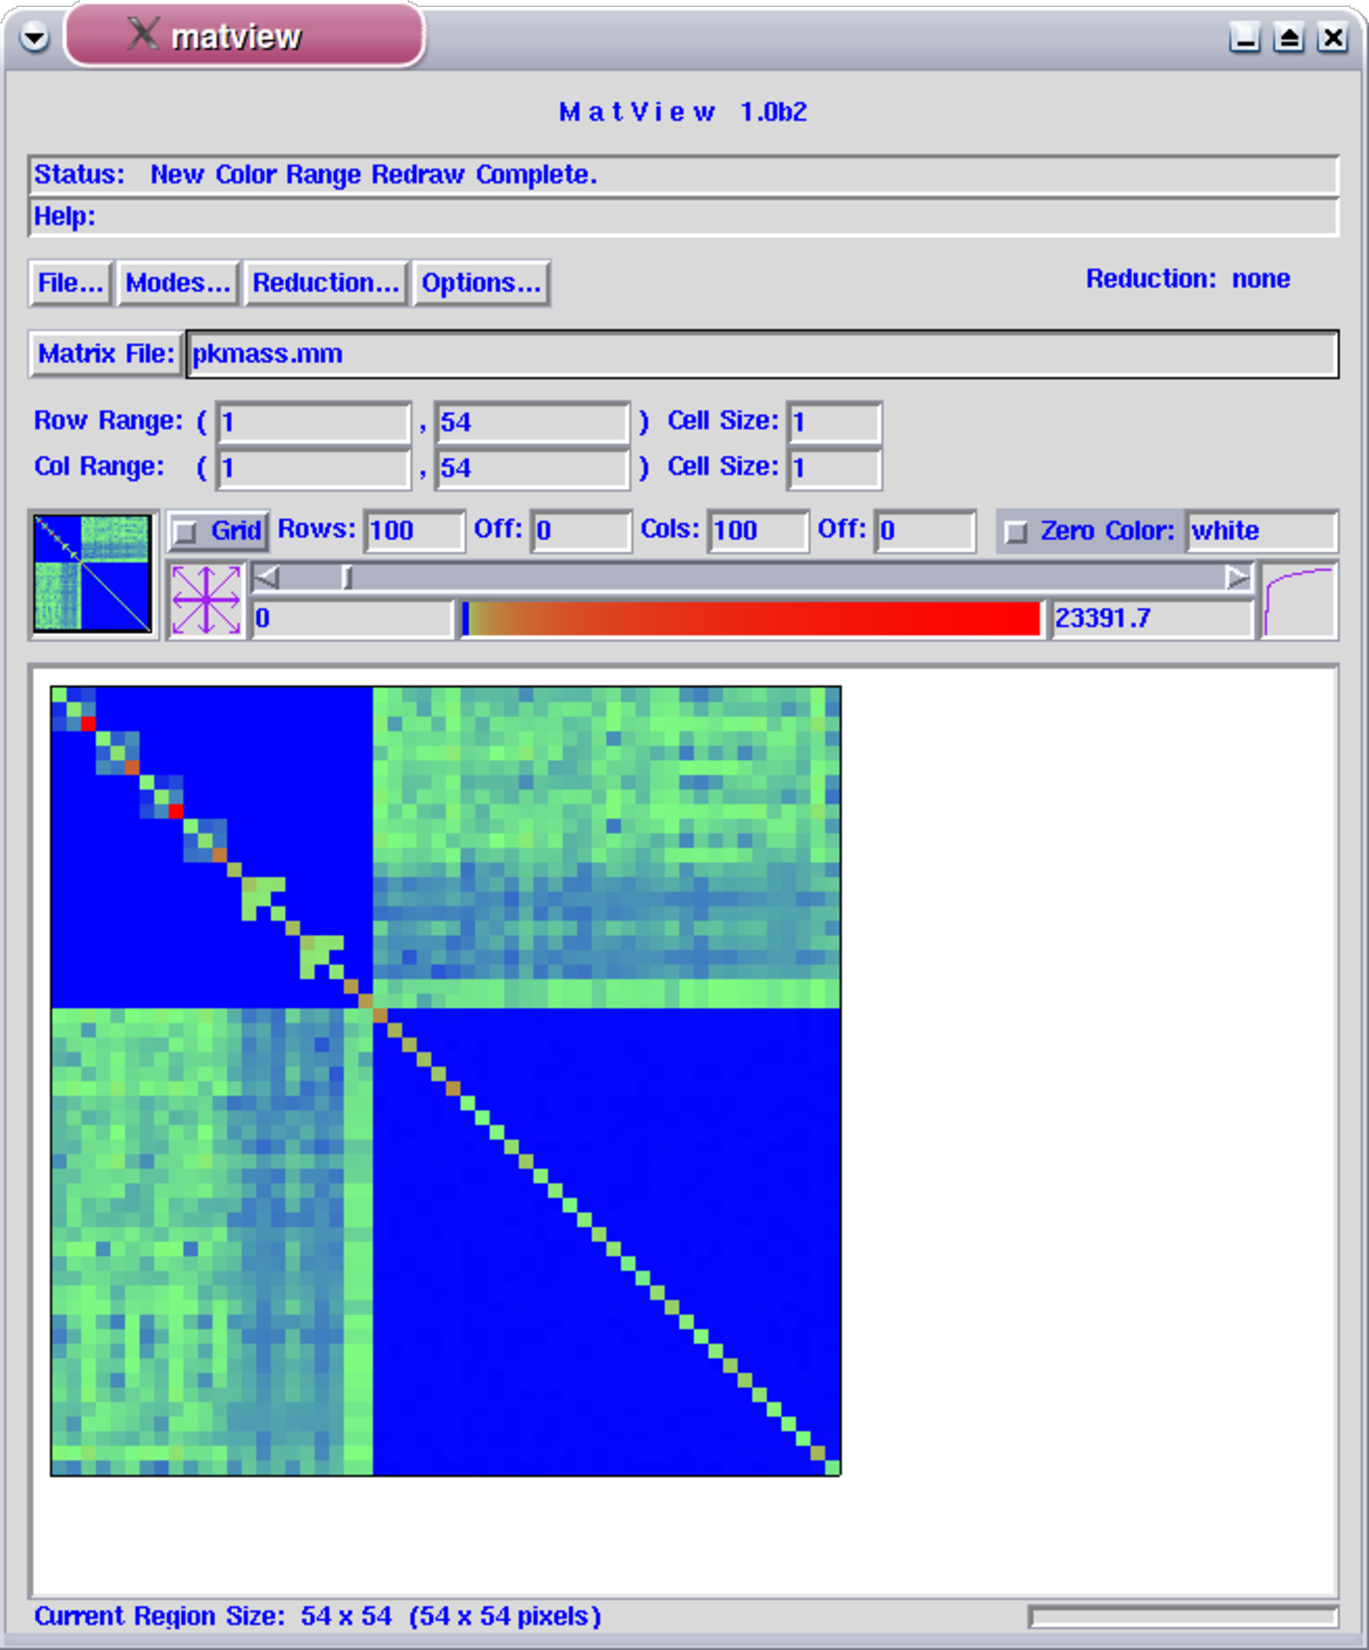
\includegraphics[height=3in,width=3.25in]{figures/manual/matview.pdf}
	\centering
	\caption{Matrix image in \Cmd{viz}}\label{fig:matview}
\end{figure}
A few capabilities of this visualization:
\begin{itemize}
	\item Clicking on an element of the matrix with the left mouse button
			displays the value of the element.
	\item Middle-clicking and dragging the mouse selects a region
			to zoom-in on, and right-clicking restores the unzoomed view.
	\item Matrix elements are colored to indicate values according
			to the color map above the matrix. A slider above the
			color map distorts the color map; this is often necessary
			to make all the non-zero elements visible.
\end{itemize}


\paragraph{Command Line Usage.} \label{ref:viz-cmdline}
Both \Cmd{viz} and \Cmd{amviz} can be used on the command line
to visualize data in \Cmd{flut}-created plotfiles,
or Universal files, respectively.
\index{viz@{\sf  viz}!command line usage} % kludge
\index{amviz!command line usage}

The options to \Code{viz} are similar to the input-file
version; the main difference is that the syntax is like
other Unix commands. For example, to plot \Code{sigma} against \Code{veas}
from a file called \Code{core.apf}:
\begin{lstlisting}
> viz -x veas -y sigma core
\end{lstlisting}
Animated-mode visualization will be available by right-clicking on
curves if visualization data was imported prior to the \Cmd{flut} function
that produced the plotfile \Sectref{sect:universal-file}.

Multiple .apf files may be specified; the number of files is only limited by
computer memory and the number of arguments allowed on a command-line by
the operating system (hundreds).

Here is a synopsis of the command-line version of \Cmd{viz}:
\begin{lstlisting}
viz [options] .apf file(s)
    -x[min:max] xpar   the name of the x-parameter; optionally, limits
                       may be given in square brackets.
    -y[min:max] list   the name(s) of the y-variable(s).  Multiple y-variables
                       can be specified using a sequence enclosed in quotes,
                       for example
                          -y 'y[1:2:12]'
                       plots y1, y2, y3, ... y12
    -c list            curve(s) to plot. Multiple curves can be specified
                       using a sequence list enclosed in quotes. For example
                         -c '[3:2:12,15]'
                       which is equivalent to
                         -c '3,5,7,9,11,15'
\end{lstlisting}
There is only one option to \Cmd{amviz}: the name (or more precisely the path)
of the Universal file (\Sectref{sect:universal-file} contains the format of
a Universal file)\index{universal-file!in amviz}.
If the name of the file ends in \Code{.uf} it is not
necessary to include the extension.

\paragraph{Examples.}
The function
\begin{lstlisting}
   viz { id=core, x=vtas, y=sigma, c{4:10} }
\end{lstlisting}
in an \Fina script will produce a plot from a previous
\Cmd{flut} run; clicking on the curves will produce
animated modes provided the required data is available
(\Sectref{sect:universal-file}), as illustrated in \Figref{fig:viz-amviz}.
\par
\begin{figure}[ht]\label{fig:viz-amviz}
		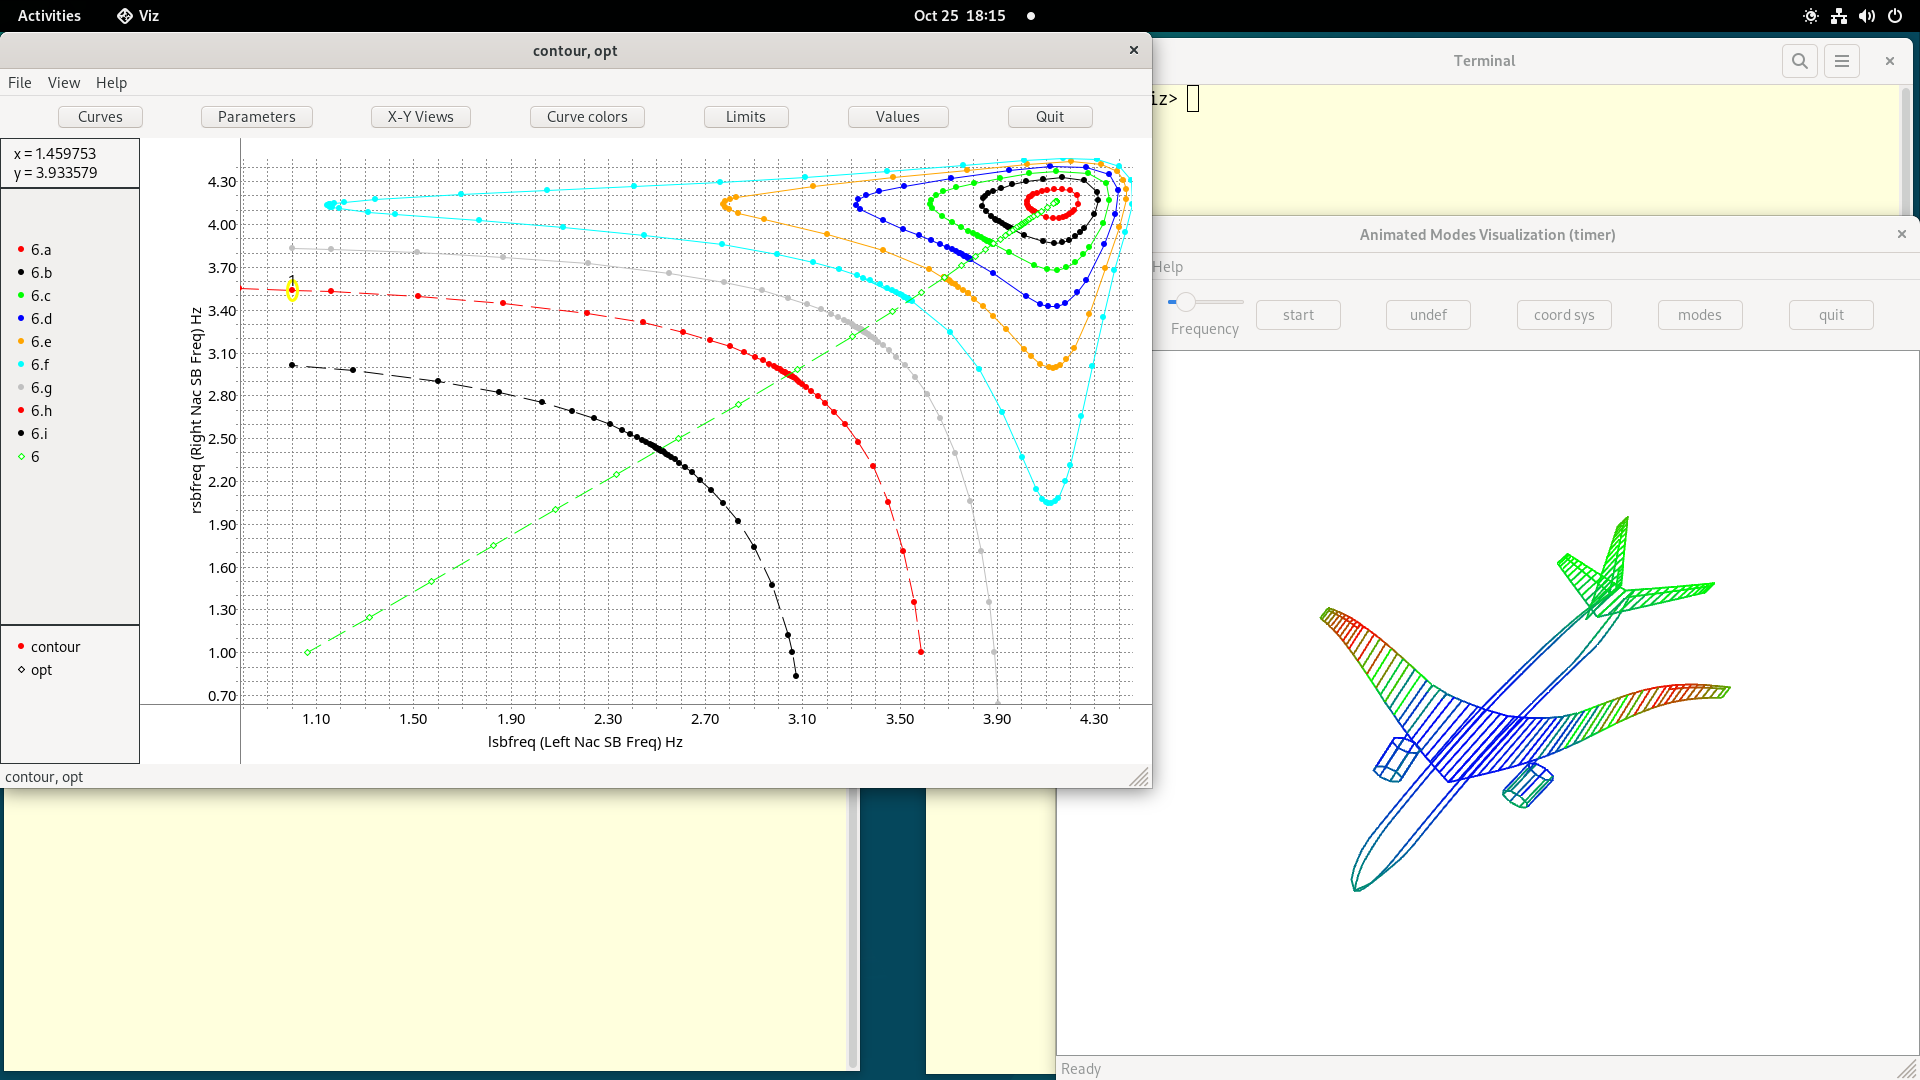
\includegraphics[height=9cm,width=16cm]{figures/manual/viz-amviz.png}
	\centering
\end{figure}
% To plot on a log scale, include the word \Spec{log} in
% the list of \Spec{x} or \Spec{y} parameters:
% \begin{lstlisting}
%    viz { id=frf, x=(freq,log), y=(pilot,log) }
% \end{lstlisting}

\paragraph{See Also}
\Fina function \Cmd{flut} (\ref{ref:flut})
        
% utility commands --------------------------------------------------------
% \section{Utility Commands}\label{sect:utility}
\Manpg{Utilities}
Several utility programs are included to aid in running \Fina;
these are run from the command line. Some are simply enhancements
to standard Unix commands, e.g. \Cmd{dtree}, \Cmd{tgrep},
and \Cmd{lspath}.
\newline

\Spec{amviz}
\begin{quote}
visualize animated modes using data contained in the specified
Universal file (\cite{UniversalFile}).
See the \Cmd{amviz} reference (\Sectref{ref:viz-cmdline})
for details on usage.
\end{quote}

\Spec{diffmm \Subst{file1.mm} \Subst{file2.mm}}
\index{diffmm}\index{difference!between matrices}
\begin{quote}
display the difference between two matrices in Matrix Market (.mm) formatted files.
\end{quote}

\Spec{dtree [-s] [\Subst{path}]}
\begin{quote}
display on stdout the directory tree rooted at the
current directory or \Subst{path} if included.
The \Cmd{-s} option prints the directory size
next to the directory name and gives a summary of the
largest directories.
\end{quote}

\Spec{lspath}
\begin{quote}
lists the directories in your current PATH, one per line
\end{quote}

\Spec{matview \Subst{file\/}}
\begin{quote}
Visualize a matrix in a file with a \Cmd{.mm} extension
(Matrix Market file \cite{matrixmarket}).
These files are produced by \Fina
functions when matrices are too large to include in the printed output.
\Cmd{matview} has a number of features which
make examining the structure and values of a matrix very easy,
including color scaling, zooming, and viewing individual matrix
elements. Figure \ref{fig:matview} shows an example of the display.
\end{quote}

\Spec{tgrep [options] \Subst{pattern} \Subst{file} [\Subst{file} ...] [\Subst{dir\/}]}
\begin{quote}
Search for patterns in specified files in a directory tree rooted at \Subst{dir}
(default: current directory). \Subst{options} are any \Code{grep} options
that do not take arguments (e.g. -e).
\end{quote}

\Spec{viz [ \Subst{options} ] }
\begin{quote}
Run a simple 2D plotter (the \Fina \Code{viz} command).
See the \Code{viz} reference (\Sectref{ref:viz-cmdline})
for details on usage.
\end{quote}

